\section*{附錄二\quad 聯立方程式求解的幾何解釋}
\addcontentsline{toc}{section}{附錄二\quad 聯立方程式求解的幾何解釋}
\label{sec:b3_a2}

\renewcommand{\thefigure}{附2-\arabic{figure}}
\setcounter{figure}{0}

設 $\mathbf{a}, \mathbf{b}, \mathbf{c}$ 為空間中的三個向量，則 $\mathbf{a}, \mathbf{b}, \mathbf{c}$ 的線性張拓
\[ \langle \mathbf{a}, \mathbf{b}, \mathbf{c} \rangle \text{ 定義為 } \{\alpha\mathbf{a} + \beta\mathbf{b} + \gamma\mathbf{c} \mid \alpha, \beta, \gamma \in \mathbf{R}\} \]
設 $\mathbf{a} = \vec{OA}, \mathbf{b} = \vec{OB}, \mathbf{c} = \vec{OC}$，則當 $O, A, B, C$ 四點不共面時 $\langle \mathbf{a}, \mathbf{b}, \mathbf{c} \rangle$ 為整個三度空間，當 $O, A, B, C$ 共面而不共線時，則 $\langle \mathbf{a}, \mathbf{b}, \mathbf{c} \rangle$ 為一平面。

若給了下面聯立方程式
\begin{equation}
\begin{cases}
a_1 x + b_1 y + c_1 z = d_1 \\
a_2 x + b_2 y + c_2 z = d_2 & (*) \\
a_3 x + b_3 y + c_3 z = d_3
\end{cases}
\end{equation}
取 $\mathbf{a} = (a_1, a_2, a_3)$，$\mathbf{b} = (b_1, b_2, b_3)$，$\mathbf{c} = (c_1, c_2, c_3)$，$\mathbf{d} = (d_1, d_2, d_3)$，則“(*)是否有解的問題”便與“是否可找到三實數 $x, y, z$ 使 $\mathbf{d}$ 表成 $x\mathbf{a} + y\mathbf{b} + z\mathbf{c}$”的問題等價，亦即與“是否 $\mathbf{d}$ 會落在 $\langle \mathbf{a}, \mathbf{b}, \mathbf{c} \rangle$ 之上”的問題等價。

設
\[
\Delta = \begin{vmatrix} a_1 & b_1 & c_1 \\ a_2 & b_2 & c_2 \\ a_3 & b_3 & c_3 \end{vmatrix}, \qquad
\Delta_x = \begin{vmatrix} d_1 & b_1 & c_1 \\ d_2 & b_2 & c_2 \\ d_3 & b_3 & c_3 \end{vmatrix},
\]
\[
\Delta_y = \begin{vmatrix} a_1 & d_1 & c_1 \\ a_2 & d_2 & c_2 \\ a_3 & d_3 & c_3 \end{vmatrix}, \qquad
\Delta_z = \begin{vmatrix} a_1 & b_1 & d_1 \\ a_2 & b_2 & d_2 \\ a_3 & b_3 & d_3 \end{vmatrix}
\]

\noindent\textbf{請仔細答覆下列各題（累積計分）}

\begin{enumerate}[(1), leftmargin=2em]
  \item 定義 $\langle \mathbf{a}, \mathbf{b} \rangle = \{\alpha\mathbf{a} + \beta\mathbf{b} \mid \alpha, \beta \in \mathbf{R}\}$，則 $\mathbf{a} = -3\mathbf{b} \neq \mathbf{0}$ 時
  \begin{enumerate}[\textcircled{1}, leftmargin=2em]
    \item $\langle \mathbf{a}, \mathbf{b} \rangle$ 為整個三度空間
    \item $\langle \mathbf{a}, \mathbf{b} \rangle$ 為一平面
    \item $\langle \mathbf{a}, \mathbf{b} \rangle$ 為一直線
    \item $\langle \mathbf{a}, \mathbf{b} \rangle$ 在一平面中
    \item $\langle \mathbf{a}, \mathbf{b} \rangle$ 為一點
  \end{enumerate}

  \item $\Delta \neq 0$ 則
  \begin{enumerate}[\textcircled{1}, leftmargin=2em]
    \item $\langle \mathbf{a}, \mathbf{b}, \mathbf{c} \rangle$ 為整個三度空間
    \item $\langle \mathbf{a}, \mathbf{b}, \mathbf{c} \rangle$ 為一平面
    \item $\langle \mathbf{a}, \mathbf{b} \rangle$ 為一平面
    \item $\langle \mathbf{a}, \mathbf{b}, \mathbf{c} \rangle$ 為一點
    \item 上述答案皆不為 $\Delta \neq 0$ 之必要條件
  \end{enumerate}

  \item $\Delta \neq 0$ 則
  \begin{enumerate}[\textcircled{1}, leftmargin=2em]
    \item (*) 無解
    \item (*) 有唯一解
    \item (*) 的解自由度為 1
    \item (*) 的解自由度為 2
    \item 不能確定有解與否
  \end{enumerate}

  \item 當 $\langle \mathbf{a}, \mathbf{b}, \mathbf{c} \rangle$ 是一平面時
  \begin{enumerate}[\textcircled{1}, leftmargin=2em]
    \item (*) 無解
    \item (*) 有唯一解
    \item (*) 的解自由度為 1（即有一參數）
    \item (*) 的解自由度為 2
    \item 尚不能確定 (*) 有解與否
  \end{enumerate}

  \item $\Delta = 0$ 的幾何意思是
  \begin{enumerate}[\textcircled{1}, leftmargin=2em]
    \item $\langle \mathbf{a}, \mathbf{b}, \mathbf{c} \rangle$ 是整個三度空間
    \item $\langle \mathbf{a}, \mathbf{b}, \mathbf{c} \rangle$ 可能是一平面
    \item $\langle \mathbf{a}, \mathbf{b}, \mathbf{c} \rangle$ 可能是一條直線
    \item $\langle \mathbf{a}, \mathbf{b}, \mathbf{c} \rangle$ 在一平面中
    \item 上述答案皆非
  \end{enumerate}

  \item $\Delta = 0$ 則
  \begin{enumerate}[\textcircled{1}, leftmargin=2em]
    \item (*) 無解
    \item (*) 有唯一解
    \item (*) 的解自由度為 1
    \item (*) 的解自由度為 2
    \item 不能確定有解與否
  \end{enumerate}
\end{enumerate}

\noindent\textbf{注意：}$\Delta_x = 0$ 代表 $\mathbf{d}$ 與 $\mathbf{b}, \mathbf{c}$ 共面，從這點出發繼續考慮下列各題：

\begin{enumerate}[(1), resume, leftmargin=2em]
  \item 下列三圖中各圖皆為 5 種情形之一，請按序分別排出：

  \begin{figure}[H]
  \centering
  \begin{subfigure}[b]{0.32\textwidth}
  \centering
  \begin{tikzpicture}[>=latex, scale=0.85]
    \coordinate (O) at (0,0);
    \coordinate (A) at (1.2,0.8);
    \coordinate (B) at (-0.8,-0.5);
    \coordinate (C) at (-0.3,1.3);
    \coordinate (D) at (-0.5,1.8);

    % 平行六面體虛線
    \draw[dashed, thick] (A) -- ($(A)+(B)$) -- (B);
    \draw[dashed, thick] (A) -- ($(A)+(C)$) -- (C);
    \draw[dashed, thick] ($(A)+(B)$) -- ($(A)+(B)+(C)$) -- ($(A)+(C)$);
    \draw[dashed, thick] (B) -- ($(B)+(C)$) -- (C);
    \draw[dashed, thick] ($(B)+(C)$) -- ($(A)+(B)+(C)$);

    % 向量箭頭
    \draw[->, very thick] (O) -- (A) node[below right=-1pt] {$\mathbf{a}$};
    \draw[->, very thick] (O) -- (B) node[below left=-1pt] {$\mathbf{b}$};
    \draw[->, very thick] (O) -- (C) node[above left=-1pt] {$\mathbf{c}$};
    \draw[->, very thick] ($(B)+(C)$) -- ($(B)+(C)+(0,0.8)$) node[left] {$\mathbf{d}$};
  \end{tikzpicture}
  \caption*{(i)}
  \end{subfigure}
  \hfill
  \begin{subfigure}[b]{0.32\textwidth}
  \centering
  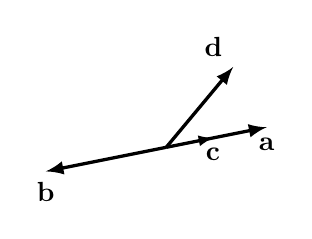
\begin{tikzpicture}[>=latex, scale=0.85]
    % 共線向量 a, b, c
    \draw[->, very thick] (0,0) -- (1.5,0.3) node[below] {$\mathbf{a}$};
    \draw[->, very thick] (0,0) -- (-1.8,-0.36) node[below] {$\mathbf{b}$};
    \draw[->, thick] (0,0) -- (0.7,0.14) node[below] {$\mathbf{c}$};

    % 獨立向量 d
    \draw[->, very thick] (0,0) -- (1.0,1.2) node[above left] {$\mathbf{d}$};
  \end{tikzpicture}
  \caption*{(ii)}
  \end{subfigure}
  \hfill
  \begin{subfigure}[b]{0.32\textwidth}
  \centering
  \begin{tikzpicture}[>=latex, scale=0.85]
    % 平面
    \draw[thick] (-1.2,-0.6) -- (1.8,-0.6) -- (2.5,1.5) -- (-0.5,1.5) -- cycle;
    \node at (2.4,0.4) [right] {\small 共面};

    % 平面內各向量
    \coordinate (O) at (0.2,-0.2);
    \draw[->, very thick] (O) -- (1.2,-0.2) node[below] {$\mathbf{a}$};
    \draw[->, very thick] (O) -- (1.0,0.6) node[right] {$\mathbf{b}$};
    \draw[->, very thick] (O) -- (-0.4,0.4) node[left] {$\mathbf{c}$};
    \draw[->, very thick] (O) -- (0.8,1.0) node[above] {$\mathbf{d}$};
  \end{tikzpicture}
  \caption*{(iii)}
  \end{subfigure}
  \caption{空間向量幾何關係示意圖}
  \label{fig:b3-a2-1}
  \end{figure}

  \begin{enumerate}[\textcircled{1}, leftmargin=2em]
    \item $\Delta = 0$ 且 $\Delta_x = \Delta_y = \Delta_z = 0$
    \item $\Delta = 0$ 且 $\Delta_x = 0, \Delta_y = 0, \Delta_z \neq 0$
    \item $\Delta \neq 0$ 且 $\Delta_x = 0, \Delta_y \neq 0, \Delta_z = 0$
    \item $\Delta = 0$ 且 $\Delta_x \neq 0, \Delta_y \neq 0, \Delta_z = 0$
    \item $\Delta \neq 0$ 且 $\Delta_x = 0, \Delta_y = 0, \Delta_z \neq 0$
  \end{enumerate}

  \item 判斷下列那幾命題正確：
  \begin{enumerate}[\textcircled{1}, leftmargin=2em]
    \item 若 $\Delta_x = \Delta_y = \Delta_z = 0$ 則 $\Delta = 0$
    \item 當 $\Delta_x = \Delta_y = \Delta_z = 0$ 時 (*) 若有解，則其解必為 $x = 0, y = 0, z = 0$
    \item 當 $\Delta \neq 0$ 時，$\Delta_x, \Delta_y, \Delta_z$ 皆不等於 0 為 (*) 有非零解的一個充分必要條件。
    \item 當 $\Delta = 0$ 時 $\Delta_x = \Delta_y = \Delta_z = 0$ 為 (*) 有解的一個必要條件。
    \item 當 $\Delta = 0$ 時 $\Delta_x = \Delta_y = \Delta_z = 0$ 為 (*) 有解的一個充分條件。
  \end{enumerate}

  \item (7) 中第 (ii) 圖

  \begin{center}
  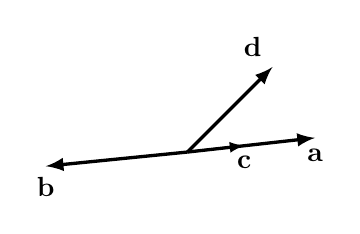
\begin{tikzpicture}[>=latex, scale=0.9]
    \draw[->, very thick] (0,0) -- (1.8,0.2) node[below] {$\mathbf{a}$};
    \draw[->, very thick] (0,0) -- (-2.0,-0.2) node[below] {$\mathbf{b}$};
    \draw[->, thick] (0,0) -- (0.8,0.09) node[below] {$\mathbf{c}$};
    \draw[->, very thick] (0,0) -- (1.2,1.2) node[above left] {$\mathbf{d}$};
  \end{tikzpicture}
  \end{center}

  可作為 (8) 中那幾命題的反例？\\
  \textbf{注意：}(9) 錯則 (10) 不給分。

  \item 下列那一種聯立方程式適合作為你 (9) 中所取那些命題的反例？請按序寫下。
  \begin{enumerate}[\textcircled{1}, leftmargin=2em]
    \item $\begin{cases} x + 2y - z = 1 \\ 3x + 6y - 3z = 3 \\ -x - 2y + z = -3 \end{cases}$
    \item $\begin{cases} x + 2y - z = 1 \\ 3x + 6y - 3z = 3 \\ -x - 2y + z = -1 \end{cases}$
    \item $\begin{cases} x + 2y - z = 1 \\ 3x + 6y - 3z = 3 \\ -x - 2y + 3z = -3 \end{cases}$
    \item $\begin{cases} x + 2y - z = 1 \\ 3x + 6y - 3z = 3 \\ -x - 2y + 3z = -1 \end{cases}$
    \item 上述各答案皆非
  \end{enumerate}
\end{enumerate}
